\section{同调群}
\sourcepage{30--31}
现在可以定义同调群了。首先必须讨论“定向”的概念。

\entry{定义}{1.6.1}设 $\sigma$ 为单形，可以是几何单形或抽象单形。若其顶点集的两种排序相差一个偶置换，则定义它们等价。若 $\dim\sigma>0$，则顶点的所有排序分成两个等价类，每个等价类称为 $\sigma$ 的一种\textbf{定向}（orientation）。若 $\sigma$ 为 $0$ 维单形，则只有一个等价类，因而只有一种定向。\textbf{定向单形}（oriented simplex）是单形 $\sigma$ 连同它的一种定向。

若点 $v_0,v_1,\ldots,v_p$ 独立，用符号 $v_0v_1\cdots v_p$ 表示它们张成的单形，用 $[v_0,v_1,\ldots,v_p]$ 表示由该单形连同排序 $(v_0,v_1,\ldots,v_p)$ 的等价类组成的定向单形。

在上下文含义明确时，偶尔也会用单个字母，例如 $\sigma$，表示单形或定向单形。

\entry{例}{1.6.2}我们常用箭头表示 $1$ 维单形的定向。定向单形 $[v_0,v_1]$ 如图 1.6.1 所示，箭头从 $v_0$ 指向 $v_1$。$2$ 维单形的定向用环形箭头表示。图中的定向单形 $[v_0,v_1,v_2]$ 用沿 $v_0$ 到 $v_1$ 再到 $v_2$ 的方向的箭头表示。可以验证，$[v_1,v_2,v_0]$ 与 $[v_2,v_0,v_1]$ 也由同一个顺时针箭头表示。逆时针箭头则表示相反定向的单形。

类似地，定向单形 $[v_0,v_1,v_2,v_3]$ 可用图中的螺旋箭头表示，这个箭头称为“右手螺旋”。如果右手四指沿 $v_0$ 到 $v_1$ 再到 $v_2$ 的方向弯曲，那么拇指指向 $v_3$。可以验证，$[v_0,v_2,v_3,v_1]$，以及与这两种排序等价的另外十种排序，也都给出右手螺旋。“左手螺旋”则表示相反的定向。
\begin{center}
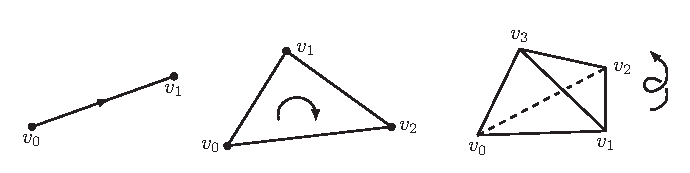
\includegraphics[width=114mm]{figures/1-6-1.pdf}\\图 1.6.1
\end{center}
\entry{定义}{1.6.3}设 $K$ 为单纯复形。$K$ 上的一条 \textbf{$p$ 维链}（$p$-chain），是从 $K$ 的定向 $p$ 维单形集到整数的函数 $c$，满足：
\begin{enumerate}[label=(\arabic*)]
\item 若 $\sigma,\sigma'$ 是同一个单形的相反定向，则 $c(\sigma)=-c(\sigma')$。
\item 除有限多个定向单形外，均有 $c(\sigma)=0$。
\end{enumerate}
通过逐点相加定义 $p$ 维链的加法；所得群记为 $C_p(K)$，称为 $K$ 的\textbf{定向 $p$ 维链群}。若 $p<0$ 或 $p>\dim K$，则令 $C_p(K)$ 为平凡群。

若 $\sigma$ 为定向单形，与它对应的\textbf{初等链}（elementary chain）是如下函数 $c$：
\[
\begin{aligned}
c(\sigma)&=1,\\
c(\sigma')&=-1&&\text{若 $\sigma'$ 是 $\sigma$ 的相反定向},\\
c(\tau)&=0&&\text{对所有其他定向单形 $\tau$}.
\end{aligned}
\]
我们常滥用记号，不仅用 $\sigma$ 表示单形或定向单形，也用它表示相应的初等 $p$ 维链。依此约定，若 $\sigma,\sigma'$ 是同一单形的相反定向，就写作 $\sigma'=-\sigma$，因为把它们解释为初等链时，这个等式成立。

\sourcepage{32--33}
\entry{引理}{1.6.4}群 $C_p(K)$ 是自由阿贝尔群。给每个 $p$ 维单形选择一种定向，相应的初等链就构成 $C_p(K)$ 的一组基。

\noindent\textbf{证明：}证明很直接。任意地给 $K$ 的每个 $p$ 维单形定向，不必参照其他单形的定向。之后，每条 $p$ 维链 $c$ 都能唯一写成相应初等链 $\sigma_i$ 的有限线性组合 $c=\sum n_i\sigma_i$。链 $c$ 在定向单形 $\sigma_i$ 上取值 $n_i$，在其相反定向上取值 $-n_i$，在未出现在此和中的所有定向 $p$ 维单形上取值 $0$。\hfill$\square$

群 $C_0(K)$ 与其他链群不同，它有一组自然的基，因为每个 $0$ 维单形只有一种定向。若 $p>0$，则 $C_p(K)$ 没有“自然”的基，因为必须任意地给各 $p$ 维单形定向，才能得到一组基。

\entry{推论}{1.6.5}从 $K$ 的定向 $p$ 维单形集到阿贝尔群 $G$ 的任意函数 $f$，只要对所有定向 $p$ 维单形满足 $f(-\sigma)=-f(\sigma)$，就能唯一扩张为同态 $C_p(K)\to G$。

\entry{定义}{1.6.6}现在定义称为\textbf{边界算子}（boundary operator）的同态
\[
\partial_p:C_p(K)\longrightarrow C_{p-1}(K).
\]
若 $\sigma=[v_0,v_1,\ldots,v_p]$ 是定向单形，且 $p>0$，定义
\[
\partial_p\sigma=\partial_p[v_0,v_1,\ldots,v_p]
=\sum_{i=0}^p(-1)^i[v_0,v_1,\ldots,\widehat v_i,\ldots,v_p].\tag{$*$}
\]
\translatornote{原文此式的符号印作 $(-1)^p$，而后面的计算和例子均使用 $(-1)^i$；这里采用与后文一致的边界公式。}
其中 $\widehat v_i$ 表示从该序列中删去顶点 $v_i$。由于 $p<0$ 时 $C_p(K)$ 为平凡群，故当 $p\leq0$ 时，$\partial_p$ 为平凡同态。

必须检验 $\partial_p$ 是良定义的。具体地，需要证明 $\partial_p(-\sigma)=-\partial_p(\sigma)$。为此，只需证明：若交换 $[v_0,\ldots,v_p]$ 中两个相邻顶点，$(*)$ 右边就改变符号。比较
\[
\partial_p[v_0,\ldots,v_j,v_{j+1},\ldots,v_p],\qquad
\partial_p[v_0,\ldots,v_{j+1},v_j,\ldots,v_p].
\]
分别展开为四部分，得到
\begin{align*}
\partial_p\sigma={}&\sum_{i<j}(-1)^i[v_0,\ldots,\widehat v_i,\ldots,v_{j-1},v_j,v_{j+1},v_{j+2},\ldots,v_p] &&\text{(a)}\\
&+\sum_{i>j+1}(-1)^i[v_0,\ldots,v_{j-1},v_j,v_{j+1},v_{j+2},\ldots,\widehat v_i,\ldots,v_p] &&\text{(b)}\\
&+(-1)^j[v_0,\ldots,v_{j-1},v_{j+1},v_{j+2},\ldots,v_p] &&\text{(c)}\\
&+(-1)^{j+1}[v_0,\ldots,v_{j-1},v_j,v_{j+2},\ldots,v_p]. &&\text{(d)}
\end{align*}
\begin{align*}
\partial_p(-\sigma)={}&\sum_{i<j}(-1)^i[v_0,\ldots,\widehat v_i,\ldots,v_{j-1},v_{j+1},v_j,v_{j+2},\ldots,v_p] &&\text{(a$'$)}\\
&+\sum_{i>j+1}(-1)^i[v_0,\ldots,v_{j-1},v_{j+1},v_j,v_{j+2},\ldots,\widehat v_i,\ldots,v_p] &&\text{(b$'$)}\\
&+(-1)^j[v_0,\ldots,v_{j-1},v_j,v_{j+2},\ldots,v_p] &&\text{(c$'$)}\\
&+(-1)^{j+1}[v_0,\ldots,v_{j-1},v_{j+1},v_{j+2},\ldots,v_p]. &&\text{(d$'$)}
\end{align*}
(a$'$) 行右边是 (a) 行右边的负值，因为只交换了 $v_j,v_{j+1}$，其他顶点位置不变。同样，(b$'$) 是 (b) 的负值。(c$'$) 是 (d) 的负值，因为顶点顺序相同，而 $-1$ 的指数相差 $1$；同样，(d$'$) 是 (c) 的负值。这就验证了 $\partial_p(-\sigma)=-\partial_p(\sigma)$。

\entry{例}{1.6.7}对于 $1$ 维单形，$\partial_1[v_0,v_1]=v_1-v_0$。对于 $2$ 维单形，
\[
\partial_2[v_0,v_1,v_2]=[v_1,v_2]-[v_0,v_2]+[v_0,v_1].
\]
对于 $3$ 维单形，
\[
\partial_3[v_0,v_1,v_2,v_3]
=[v_1,v_2,v_3]-[v_0,v_2,v_3]+[v_0,v_1,v_3]-[v_0,v_1,v_2].
\]
图 1.6.2 展示了这些公式的几何内容。如果还记得微积分中学过的 Green 定理、Stokes 定理与 Gauss 定理的各种形式，这些图应当相当熟悉。
\begin{center}
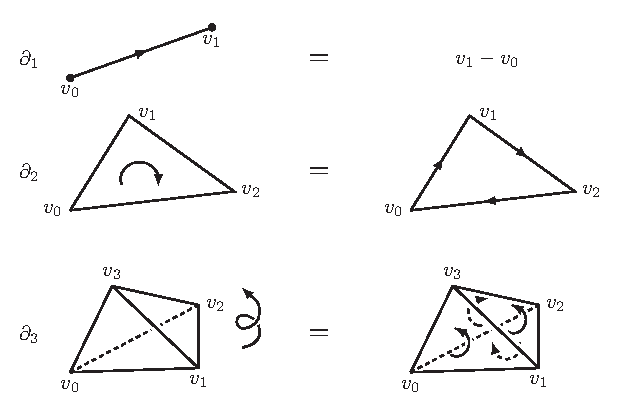
\includegraphics[width=106mm]{figures/1-6-2.pdf}\\图 1.6.2
\end{center}
\entry{例}{1.6.8}考虑图 1.6.2 中的 $1$ 维链 $\partial_2[v_0,v_1,v_2]$。对它作用算子 $\partial_1$，结果为零：每个顶点既是某条边的起点，又是另一条边的终点，因此所有项都抵消了。可以验证，计算 $\partial_2\partial_3[v_0,v_1,v_2,v_3]$ 时也发生类似的抵消。

\sourcepage{34--35}
例 1.6.8 的计算说明了下面的一般事实。

\entry{引理}{1.6.9}对于每个整数 $p$，都有 $\partial_{p-1}\circ\partial_p=0$。

\noindent\textbf{证明：}设 $0<p\leq\dim K$，否则结论平凡。设 $[v_0,\ldots,v_p]$ 为 $K$ 的定向单形，计算得
\begin{align*}
\partial_{p-1}\partial_p[v_0,\ldots,v_p]
&=\partial_{p-1}\left(\sum_{i=0}^p(-1)^i[v_0,\ldots,\widehat v_i,\ldots,v_p]\right)\\
&=\sum_{i=0}^p(-1)^i\partial_{p-1}[v_0,\ldots,\widehat v_i,\ldots,v_p]\\
&=\sum_{i=0}^p\sum_{j<i}(-1)^i(-1)^j[v_0,\ldots,\widehat v_j,\ldots,\widehat v_i,\ldots,v_p]\\
&\quad+\sum_{i=0}^p\sum_{j>i}(-1)^i(-1)^{j-1}[v_0,\ldots,\widehat v_i,\ldots,\widehat v_j,\ldots,v_p].
\end{align*}
这两个和中的各项两两抵消。\hfill$\square$

\entry{定义}{1.6.10}同态 $\partial_p:C_p(K)\to C_{p-1}(K)$ 的核称为 \textbf{$p$ 维闭链群}（group of $p$-cycles），记作 $Z_p(K)$。［字母 Z 来自德语 Zyklus；字母 C 已被用于链。］同态 $\partial_{p+1}:C_{p+1}(K)\to C_p(K)$ 的像称为 \textbf{$p$ 维边界链群}（group of $p$-boundaries），记作 $B_p(K)$。由前一引理，$(p+1)$ 维链的边界自动是 $p$ 维闭链，即 $B_p(K)\subset Z_p(K)$。定义
\[
H_p(K)=Z_p(K)/B_p(K),
\]
称此商群为 $K$ 的\textbf{第 $p$ 同调群}。

下面计算几个例子。

\entry{例}{1.6.11}考虑图 1.6.3 的复形 $K$，其底空间是边为 $e_1,e_2,e_3,e_4$ 的正方形边界。群 $C_1(K)$ 是秩为 $4$ 的自由阿贝尔群；一般的 $1$ 维链为 $c=\sum n_i e_i$。计算 $\partial_1c$，发现它在顶点 $v$ 上取值 $n_1-n_2$。对其他顶点作类似论证，可知 $c$ 为闭链，当且仅当 $n_1=n_2=n_3=n_4$。所以 $Z_1(K)$ 是由 $e_1+e_2+e_3+e_4$ 生成的无限循环群。由于 $K$ 没有 $2$ 维单形，$B_1(K)$ 平凡。因此
\[
H_1(K)=Z_1(K)/B_1(K)\cong\Z.
\]
\begin{center}
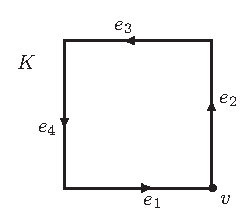
\includegraphics[width=44mm]{figures/1-6-3.pdf}\\图 1.6.3
\end{center}
\entry{例}{1.6.12}考虑图 1.6.4 中的复形 $L$，其底空间为正方形区域，既包括边界，也包括内部。一般的 $1$ 维链为 $c=\sum n_i e_i$。像前例一样推理，可知此链为闭链，当且仅当 $n_1=n_2$、$n_3=n_4$ 且 $n_5=n_3-n_2$。任意指定 $n_2,n_3$ 后，其他系数都随之确定。因此，$Z_1(L)$ 是秩为 $2$ 的自由阿贝尔群。一组可选的基是：取 $n_2=1,n_3=0$ 得到的链 $e_1+e_2-e_5$，以及取 $n_2=0,n_3=1$ 得到的链 $e_3+e_4+e_5$。这组基很方便，因为
\[
\partial_2\sigma_1=e_1+e_2-e_5,\qquad
\partial_2\sigma_2=e_3+e_4+e_5.
\]
因此 $Z_1(L)=B_1(L)$，从而
\[
H_1(L)=Z_1(L)/B_1(L)=0.
\]
\translatornote{原文该等式左边印作 $H_1(K)$，这里依本例复形名称写作 $H_1(L)$。}
还有 $H_2(L)=0$，因为 $L$ 中一般的 $2$ 维链为 $m_1\sigma_1+m_2\sigma_2$，它为闭链，当且仅当 $m_1=m_2=0$。
\begin{center}
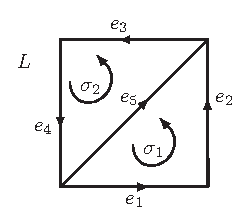
\includegraphics[width=44mm]{figures/1-6-4.pdf}\\图 1.6.4
\end{center}

\sourcepage{36--37}
这些例子或许已使你开始对同调群的几何意义有所体会。只有计算更多例子，才能开始“看见”同调类是什么。我们希望，当你对同调的几何意义有所体会之后，就会开始相信目前还远不清楚的事实：复形 $K$ 的同调群实际上只依赖于底空间 $|K|$。

再来看一个例子，其中单形的数量比前面更多。一般地，单形越多，计算闭链群 $Z_p$ 和边界链群 $B_p$ 就越繁琐。通过跳过这两个群的具体计算，直接计算同调群 $H_p$，可以缩短部分计算过程。

这里仅讨论 $p>0$ 时的群 $H_p(K)$，把 $H_0(K)$ 留到第 1.8 节。

需要引入一些术语。若链 $c$ 在每个不属于子复形 $L$ 的单形上都取值 $0$，则称 $c$ \textbf{由 $L$ 承载}（carried by $L$）。若对于某条 $(p+1)$ 维链 $d$，有 $c-c'=\partial_{p+1}d$，则称两条 $p$ 维链 $c,c'$ \textbf{同调}（homologous）。特别地，若 $c=\partial_{p+1}d$，则称 $c$ \textbf{同调于零}，或简称 $c$ \textbf{是边界}（bounds）。

\entry{例}{1.6.13}考虑图 1.6.5 的复形 $M$，其底空间为正方形区域。我们不具体计算 $1$ 维闭链群，而作如下推理。给定 $1$ 维链 $c$，设其在 $e_1$ 上的值为 $a$。直接计算可得，链
\[
c_1=c+\partial_2(a\sigma_1)
\]
在定向单形 $e_1$ 上取值 $0$。直观地说，通过给 $c$ 加上一个边界，我们已“把它从 $e_1$ 上推开”。接着类似地把 $c_1$ 从 $e_2$ 上推开：令 $b$ 为 $c_1$ 在 $e_2$ 上的值，则
\[
c_2=c_1+\partial_2(b\sigma_2)
\]
在 $e_2$ 上取值 $0$，在 $e_1$ 上也仍取值 $0$，因为 $\partial_2\sigma_2$ 的表达式中没有 $e_1$。再令 $d$ 为 $c_2$ 在 $e_3$ 上的值，则
\[
c_3=c_2+\partial_2(d\sigma_3)
\]
在 $e_3,e_2,e_1$ 上都取值 $0$。这样就把 $c$ 从这三条边上全部推开了。换言之，已经证明：给定 $1$ 维链 $c$，它同调于一条由图 1.6.5 所示 $M$ 的子复形承载的链 $c_3$。\translatornote{此处原文引用图 1.6.5；所说的子复形实际画在图 1.6.6 中。}
\begin{center}
\begin{minipage}{.46\textwidth}\centering
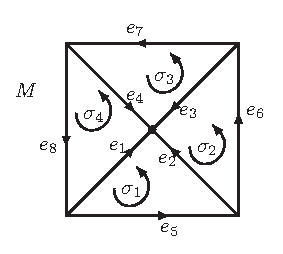
\includegraphics[width=49mm]{figures/1-6-5.pdf}\\图 1.6.5
\end{minipage}\hfill
\begin{minipage}{.46\textwidth}\centering
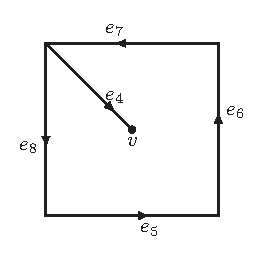
\includegraphics[width=46mm]{figures/1-6-6.pdf}\\图 1.6.6
\end{minipage}
\end{center}
现在，若 $c$ 恰为闭链，则 $c_3$ 也是闭链。因此 $c_3$ 在 $e_4$ 上的值必须为 $0$，否则 $\partial_1c_3$ 在中心顶点 $v$ 上的值便非零。于是，$M$ 中每条 $1$ 维闭链都同调于一条由正方形边界承载的闭链。由例 1.6.11 的论证可知，这样的闭链必为 $e_5+e_6+e_7+e_8$ 的某个整数倍。而后者是边界，事实上，它显然等于 $\partial_2(\sigma_1+\sigma_2+\sigma_3+\sigma_4)$。所以，如所预期，$H_1(M)=0$。

$H_2(M)=0$ 也很容易看出：与前面一样，$\sum m_i\sigma_i$ 为闭链，当且仅当所有 $m_i$ 都为零。

注意，$M$ 的同调群与例 1.6.12 中 $L$ 的同调群相同。这使我们尚未证明的断言更为可信：复形的同调群只依赖于它的底空间。

\entry{定义}{1.6.14}设 $K$ 为复形。$K$ 上的\textbf{无限 $p$ 维链}（infinite $p$-chain）是从 $K$ 的定向 $p$ 维单形集到整数的函数 $c$，满足：若 $\sigma,\sigma'$ 是同一单形的相反定向，则 $c(\sigma)=-c(\sigma')$。不再要求除有限多个单形外均有 $c(\sigma)=0$。无限 $p$ 维链群记为 $C_p^\infty(K)$；它是阿贝尔群，但一般不自由。

\sourcepage{38--39}
定义合适的边界算子 $\partial_p^\infty:C_p^\infty(K)\to C_{p-1}^\infty(K)$ 后，见习题 6，所得群
\[
H_p^\infty(K)=\ker\partial_p^\infty/\operatorname{im}\partial_{p+1}^\infty
\]
称为\textbf{基于无限链的同调群}。

下面的定义将在习题 3 中使用。

\entry{定义}{1.6.15}若一维复形的一维同调为零，则称它为\textbf{树}（tree）。\translatornote{这里保留原书的定义，其中没有要求连通；按通常术语，不连通的这种复形一般称为“森林”。}

\subsection*{习题}
\begin{enumerate}
\item 设 $\mathcal S$ 为由 $1$ 维单形 $\{v_0,v_1\},\{v_1,v_2\},\ldots,\{v_{n-1},v_n\},\{v_n,v_0\}$ 及其顶点组成的抽象复形。若 $K$ 是其几何实现，计算 $H_i(K)$。
\item 考虑图 1.6.7 中的复形 $M$；它是三个三角形与一条线段的并。计算 $H_1(M)$ 与 $H_2(M)$。
\begin{center}
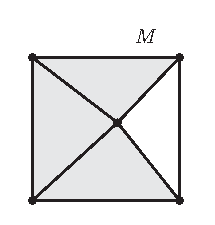
\includegraphics[width=43mm]{figures/1-6-7.pdf}\\图 1.6.7
\end{center}
\item 图 1.6.8 中的两个复形，是否有一个是树？
\begin{center}
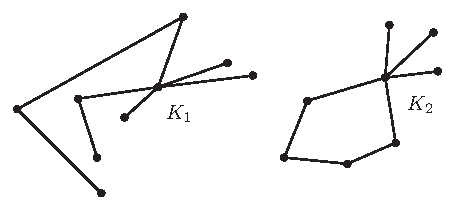
\includegraphics[width=87mm]{figures/1-6-8.pdf}\\图 1.6.8
\end{center}
\item 设 $K$ 为由某个 $3$ 维单形的所有真面组成的复形。计算 $H_1(K)$ 与 $H_2(K)$。
\item 对哪些 $i$ 有 $H_i(K^{(p)})\cong H_i(K)$？
\item \begin{enumerate}[label=(\alph*)]
\item 证明：若 $K$ 局部有限，则可用前面的公式定义边界算子 $\partial_p^\infty:C_p^\infty(K)\to C_{p-1}^\infty(K)$，且引理 1.6.9 仍成立。
\item 设 $K$ 的底空间为 $\R$，顶点为所有整数。证明 $H_1(K)=0$，而 $H_1^\infty(K)\cong\Z$。
\end{enumerate}
\end{enumerate}
